\documentclass{article}

% -- packages --
\usepackage{graphicx}
\usepackage{hyperref}

% -- format --
\hypersetup{
    colorlinks=true,
    linkcolor=blue,
    filecolor=magenta,
    urlcolor=red,
}

% -- page info --
\title{Resume Points' Proof}
\author{173079001 - 1}
\date{}


% -- document --
\begin{document}
\maketitle
\tableofcontents
\newpage
\section{Scholastic Achievements}
	\subsection{GATE Rank}
		$$percentile = \frac{total candidates - myrank }{total candidates}$$
		\begin{figure}[h]
			\frame{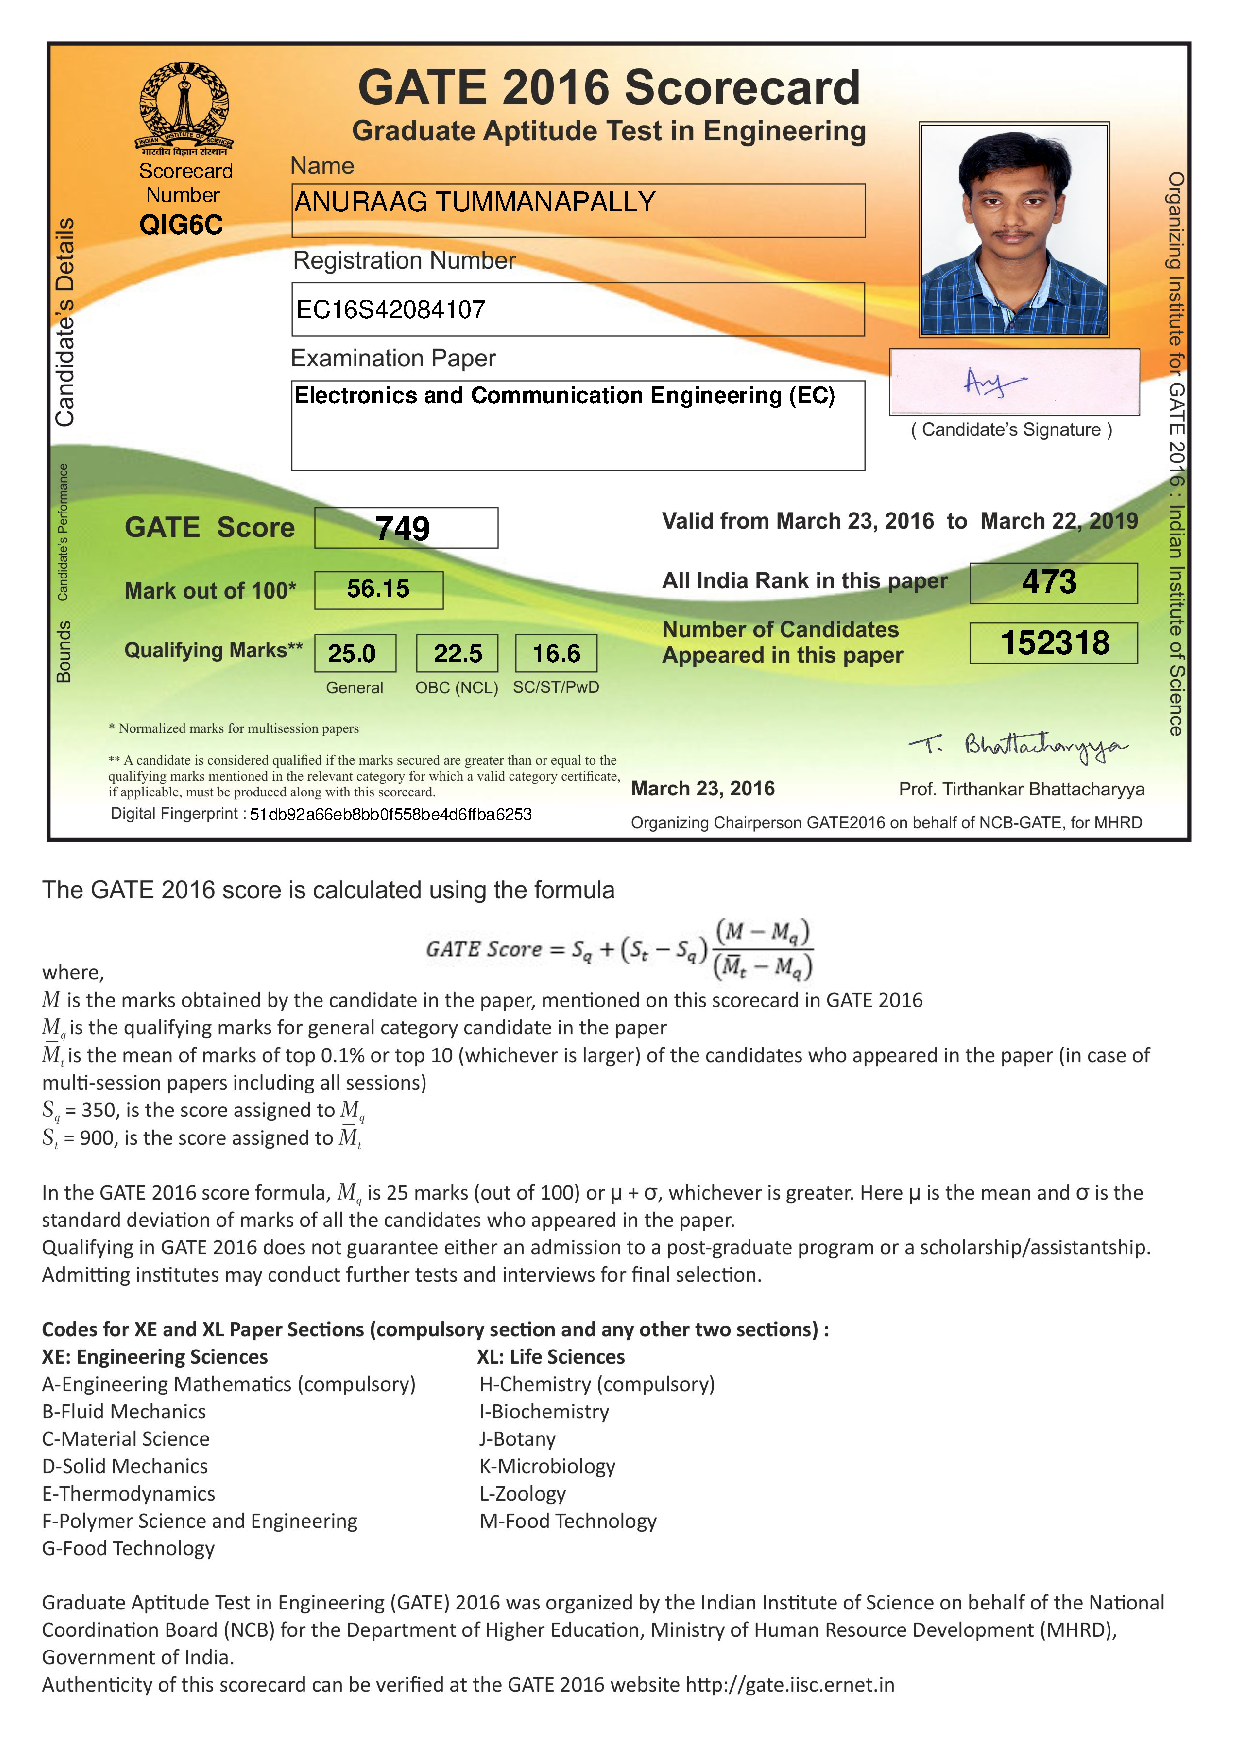
\includegraphics[trim={0 7.5cm 0 0},clip, width=\textwidth]{docs/gate_score_card.pdf}}
		\end{figure}

\newpage
	\subsection{AIEEE Rank}
		\texttt{Official URL:} \url{http://resultsarchives.nic.in/cbseresults/cbseresults2012/aieee/aieee_cbse_2012.htm}
		\begin{figure}[h]
			\frame{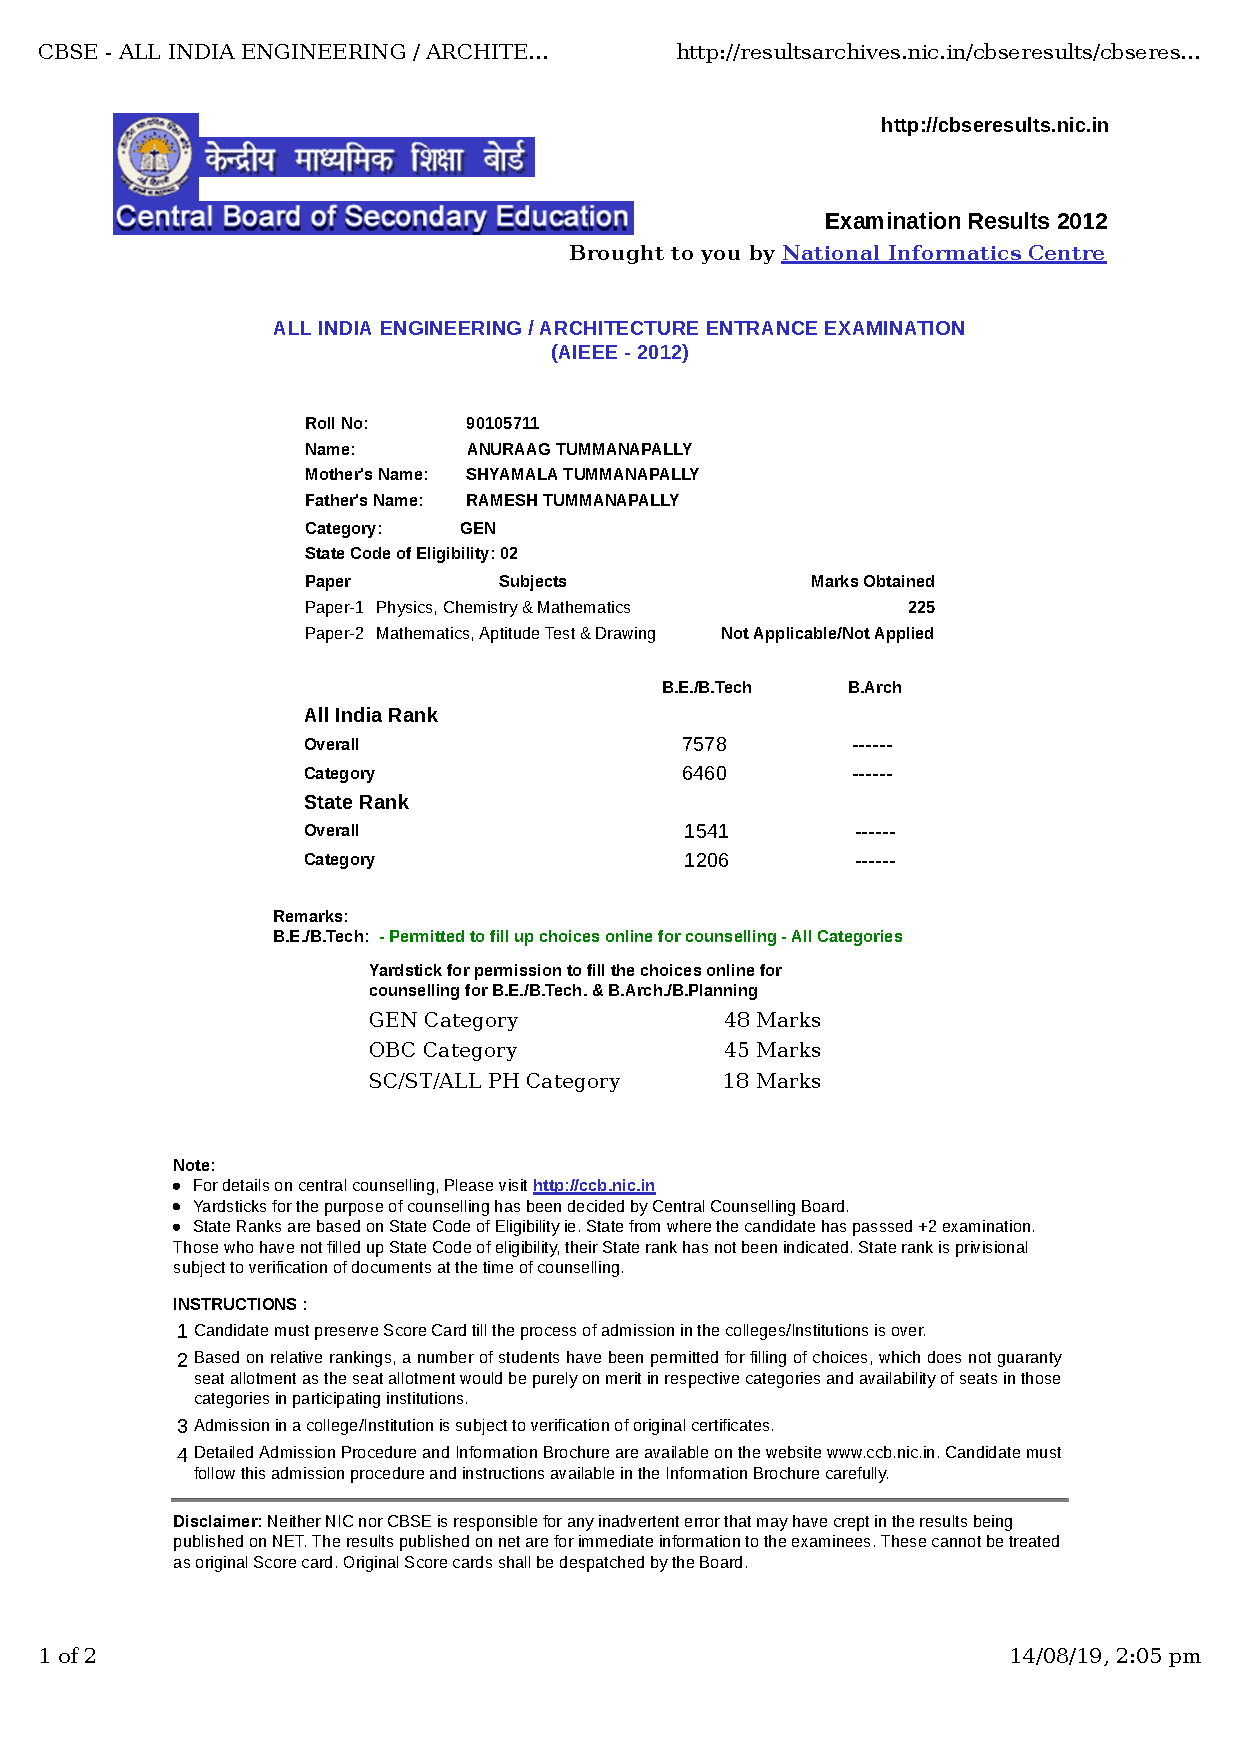
\includegraphics[trim={2cm 10.5cm 2cm 5cm},clip, width=\textwidth]{docs/aieee_rank.pdf}}
		\end{figure}
		
\newpage
	\subsection{Abacus Competition}
		\begin{figure}[h]
			\frame{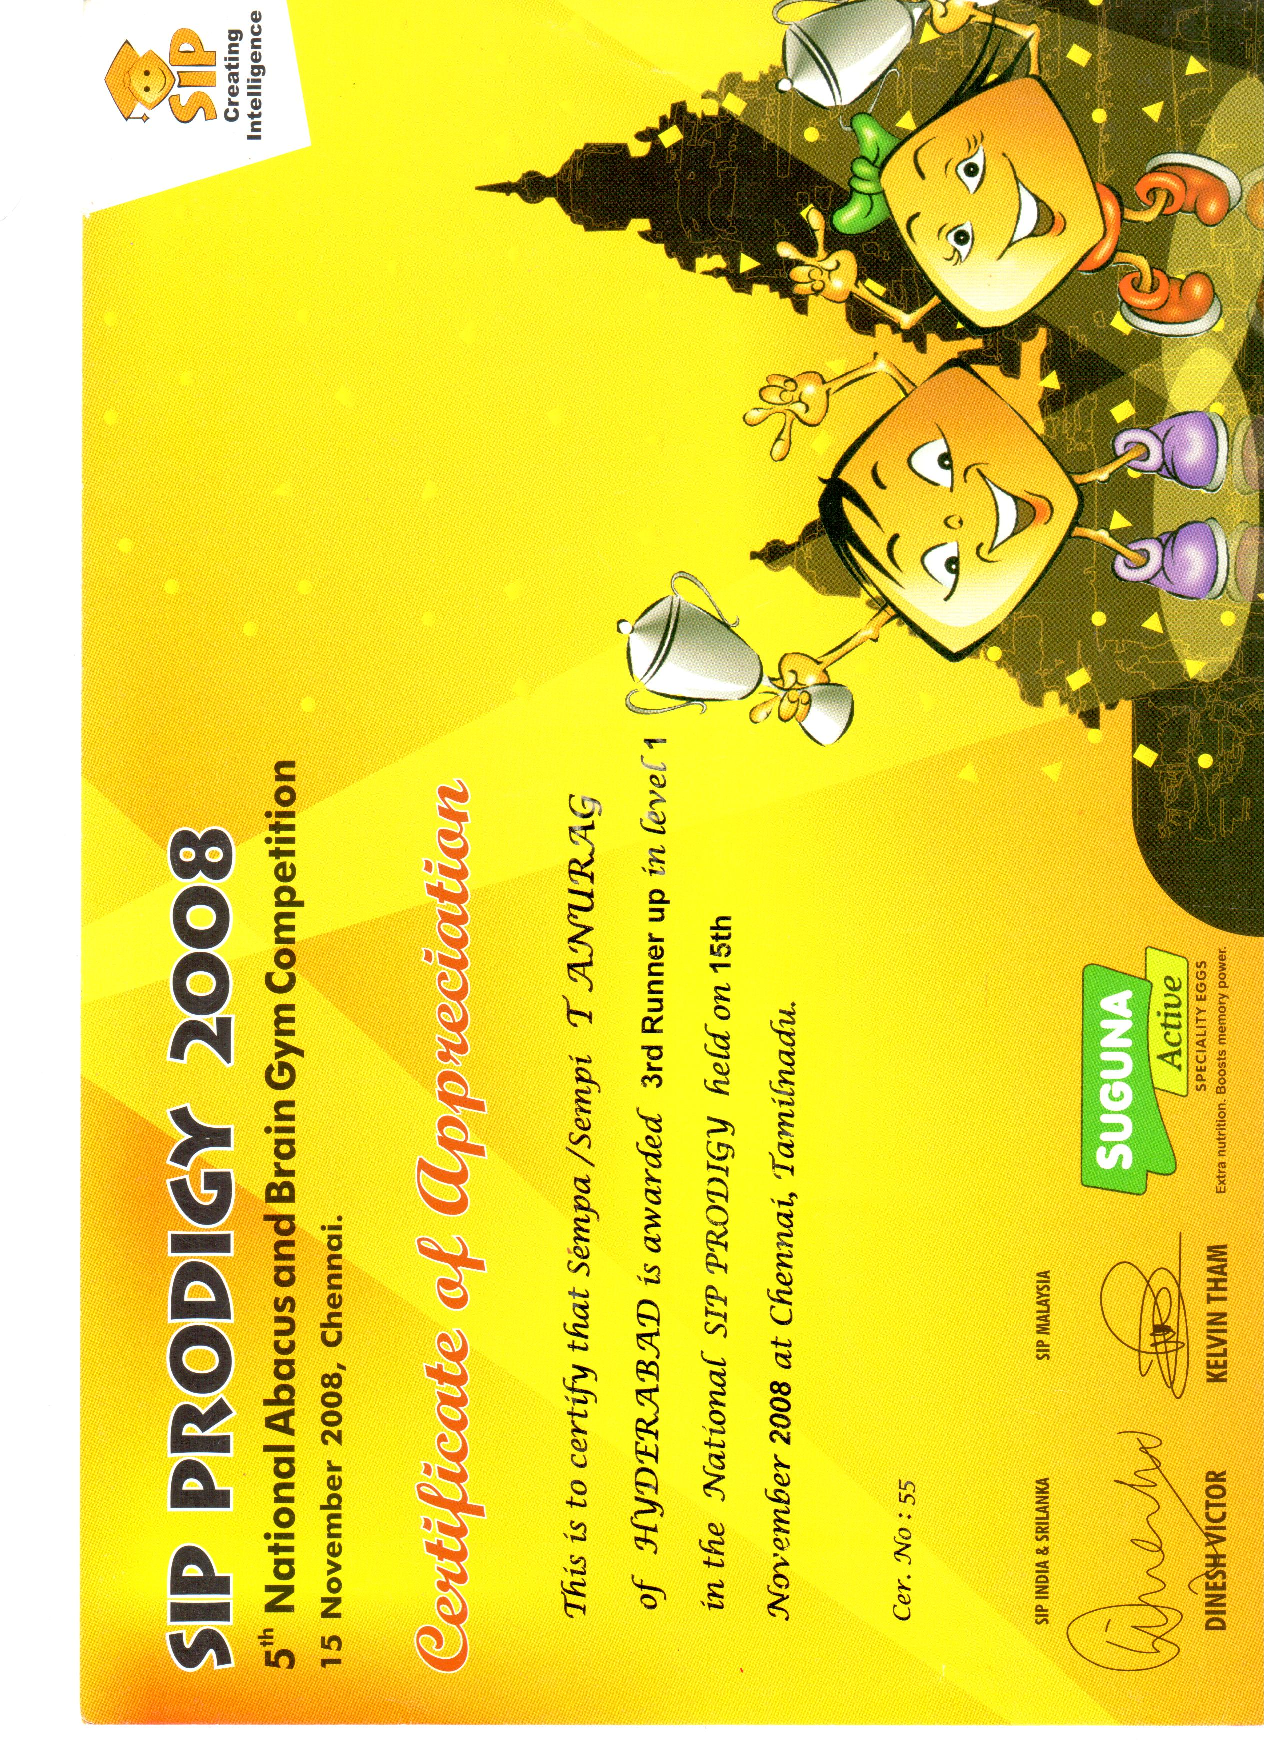
\includegraphics[trim={0 0 0 0},clip,width=0.8\textwidth]{docs/abacus.pdf}}
		\end{figure}
\newpage
\section{Major Projects and Seminar}
	\subsection{E-Mail from Guide}
		For MTP, and Seminar
		\begin{figure}[h]
			\frame{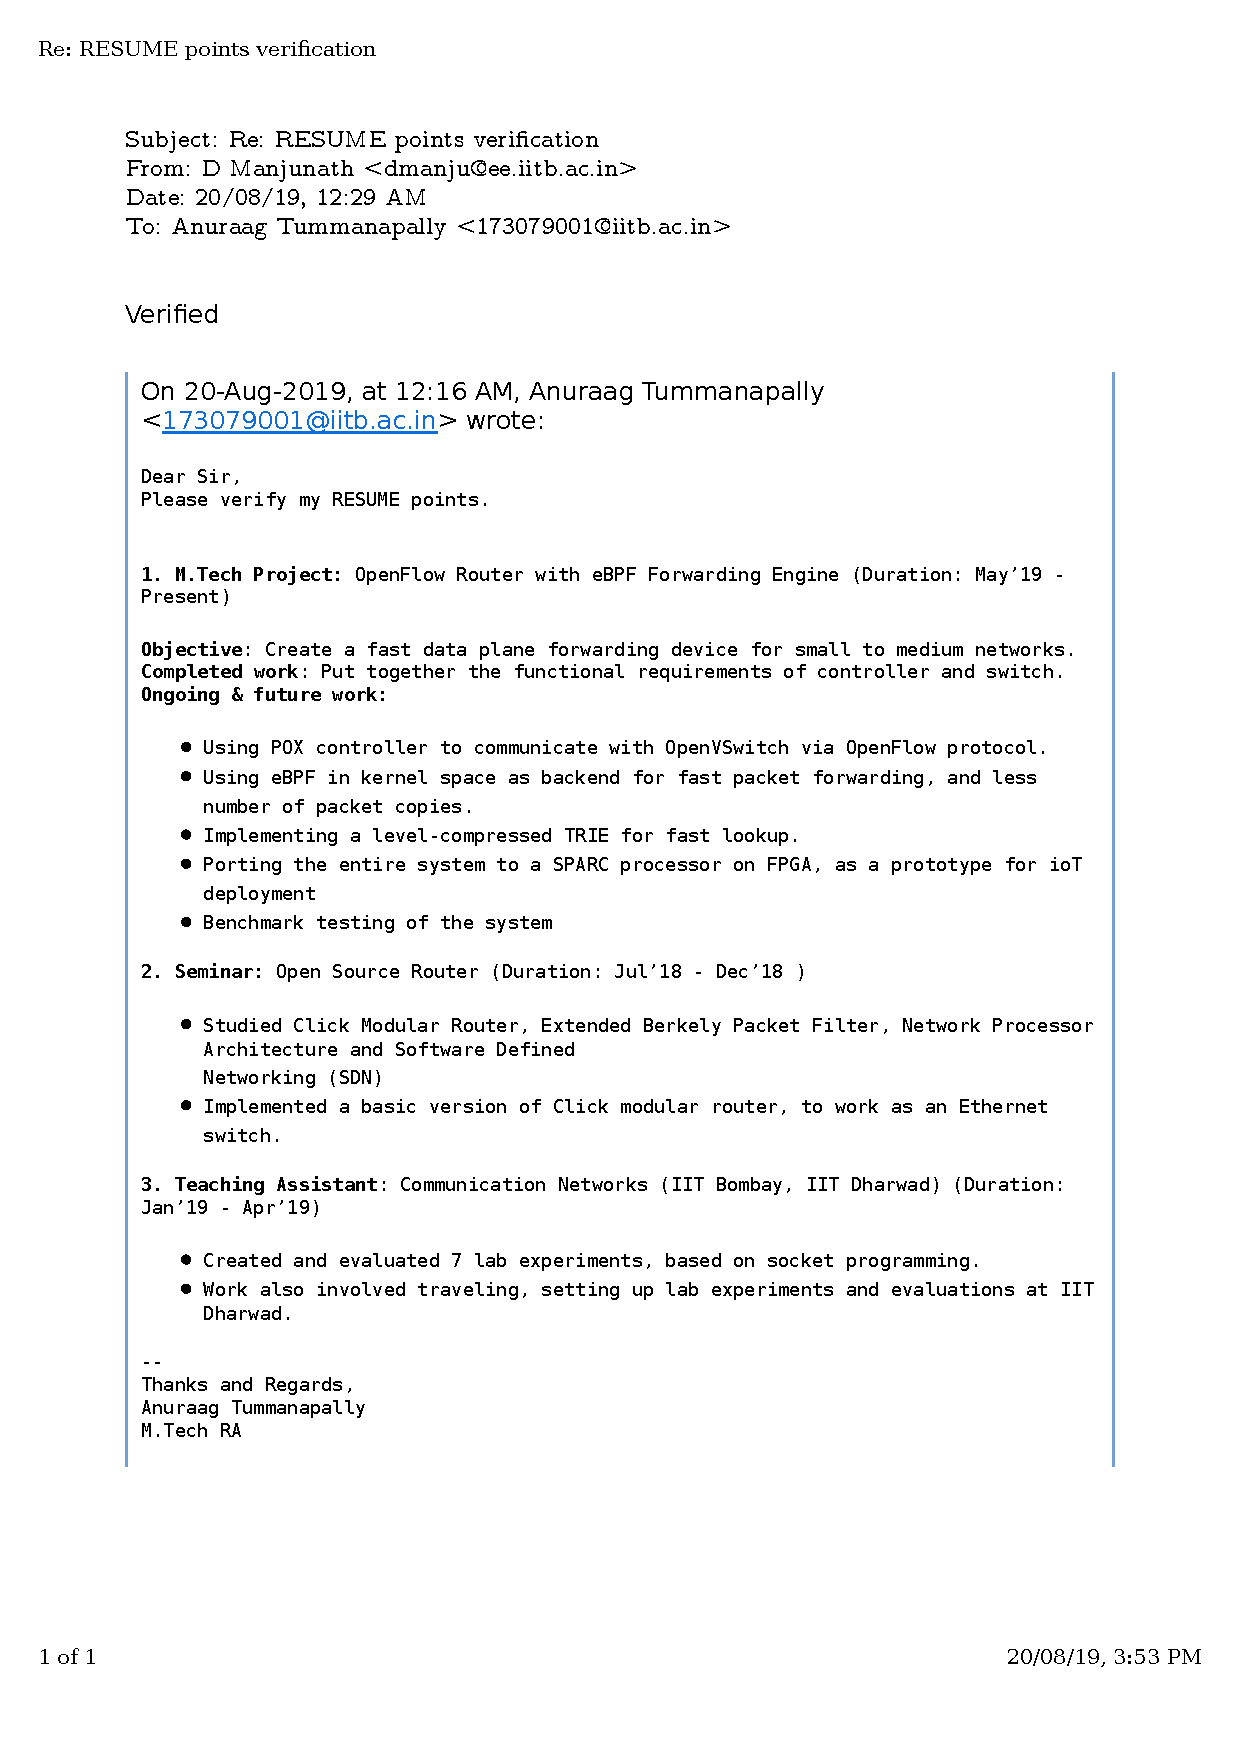
\includegraphics[trim={0 0 0 0},clip, width=0.7\textwidth]{docs/mtp_guide.pdf}}
		\end{figure}
\newpage
\section{Work Experience}
	\subsection{E-Mail from Instructor}
		For TA Work
		\begin{figure}[h]
			\frame{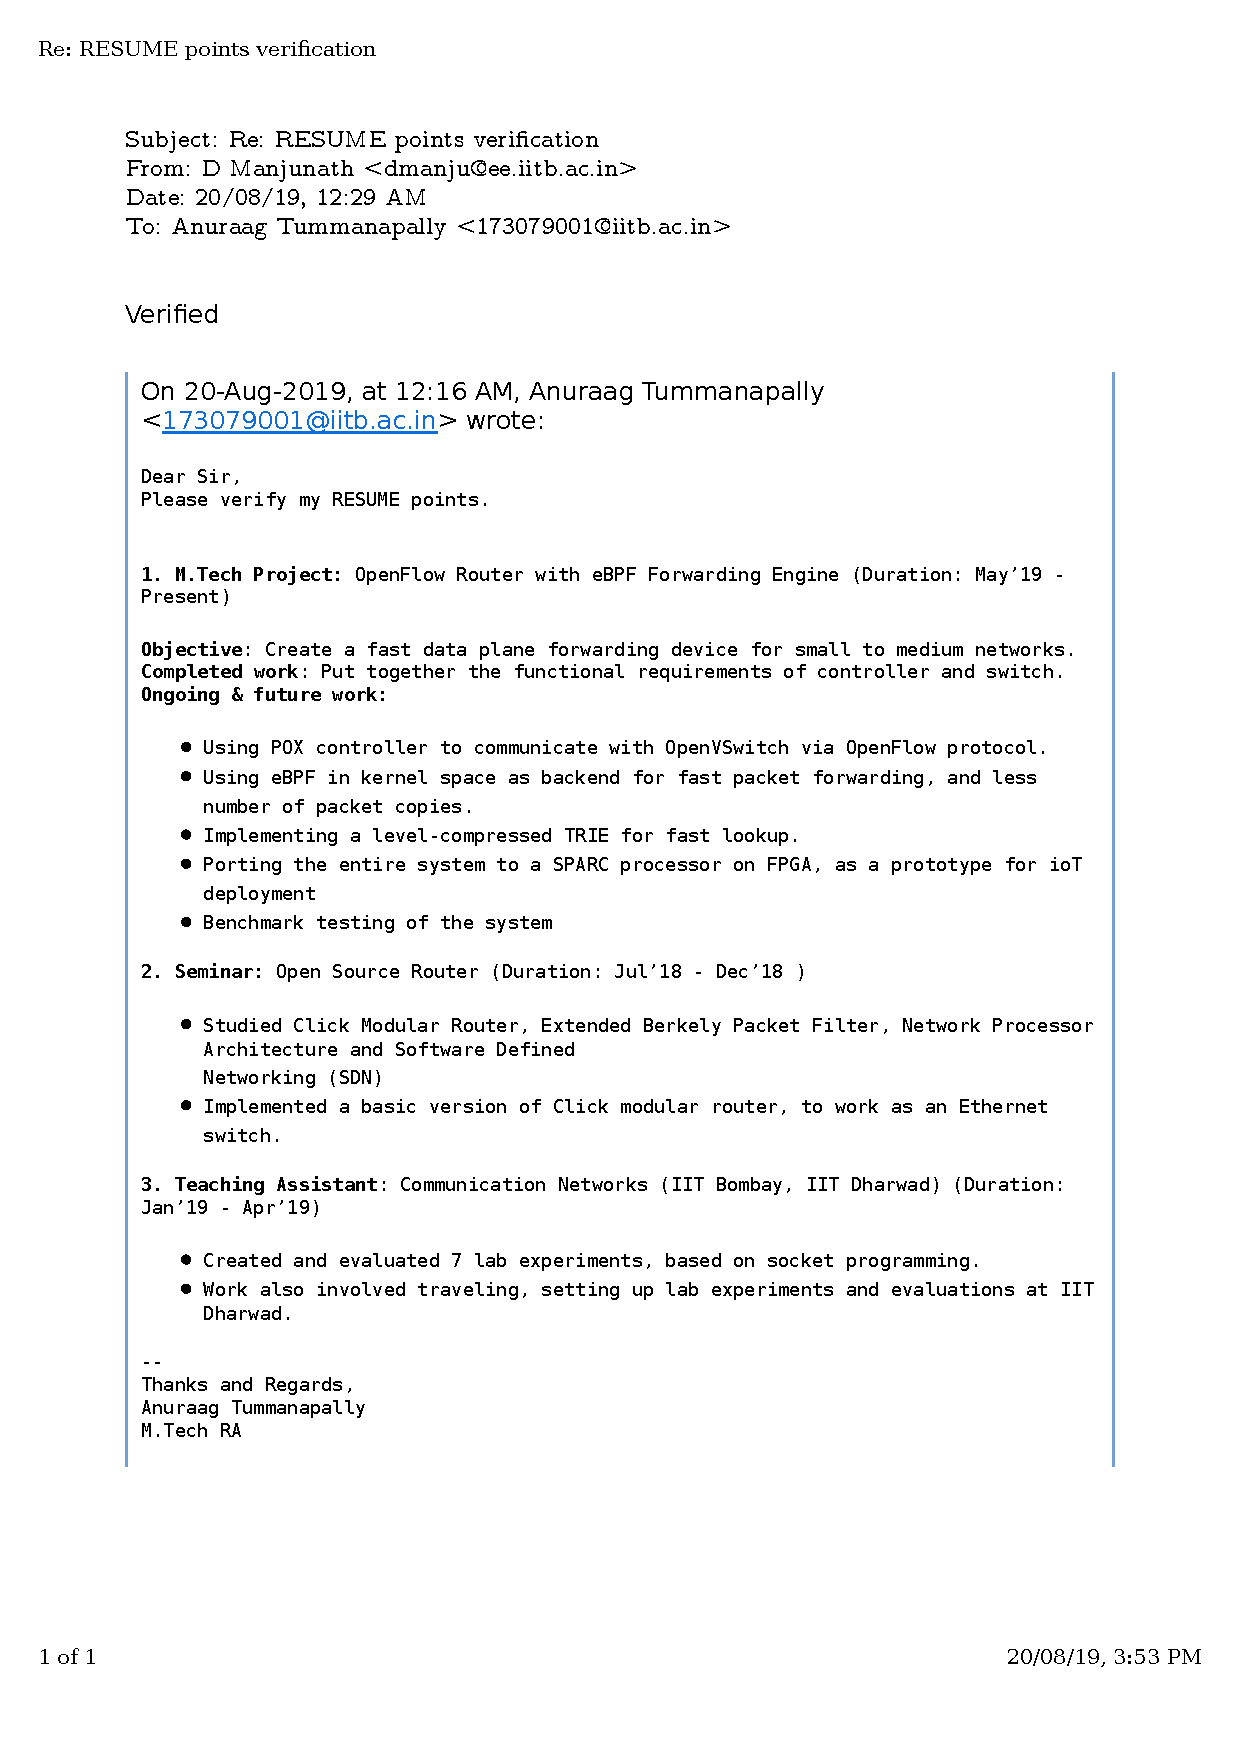
\includegraphics[trim={0 0 0 0},clip, width=0.7\textwidth]{docs/mtp_guide.pdf}}
		\end{figure}
\newpage
	\subsection{E-Mail from Lab Incharge}
		For SysAd in Electrical Department
		\begin{figure}[h]
			\frame{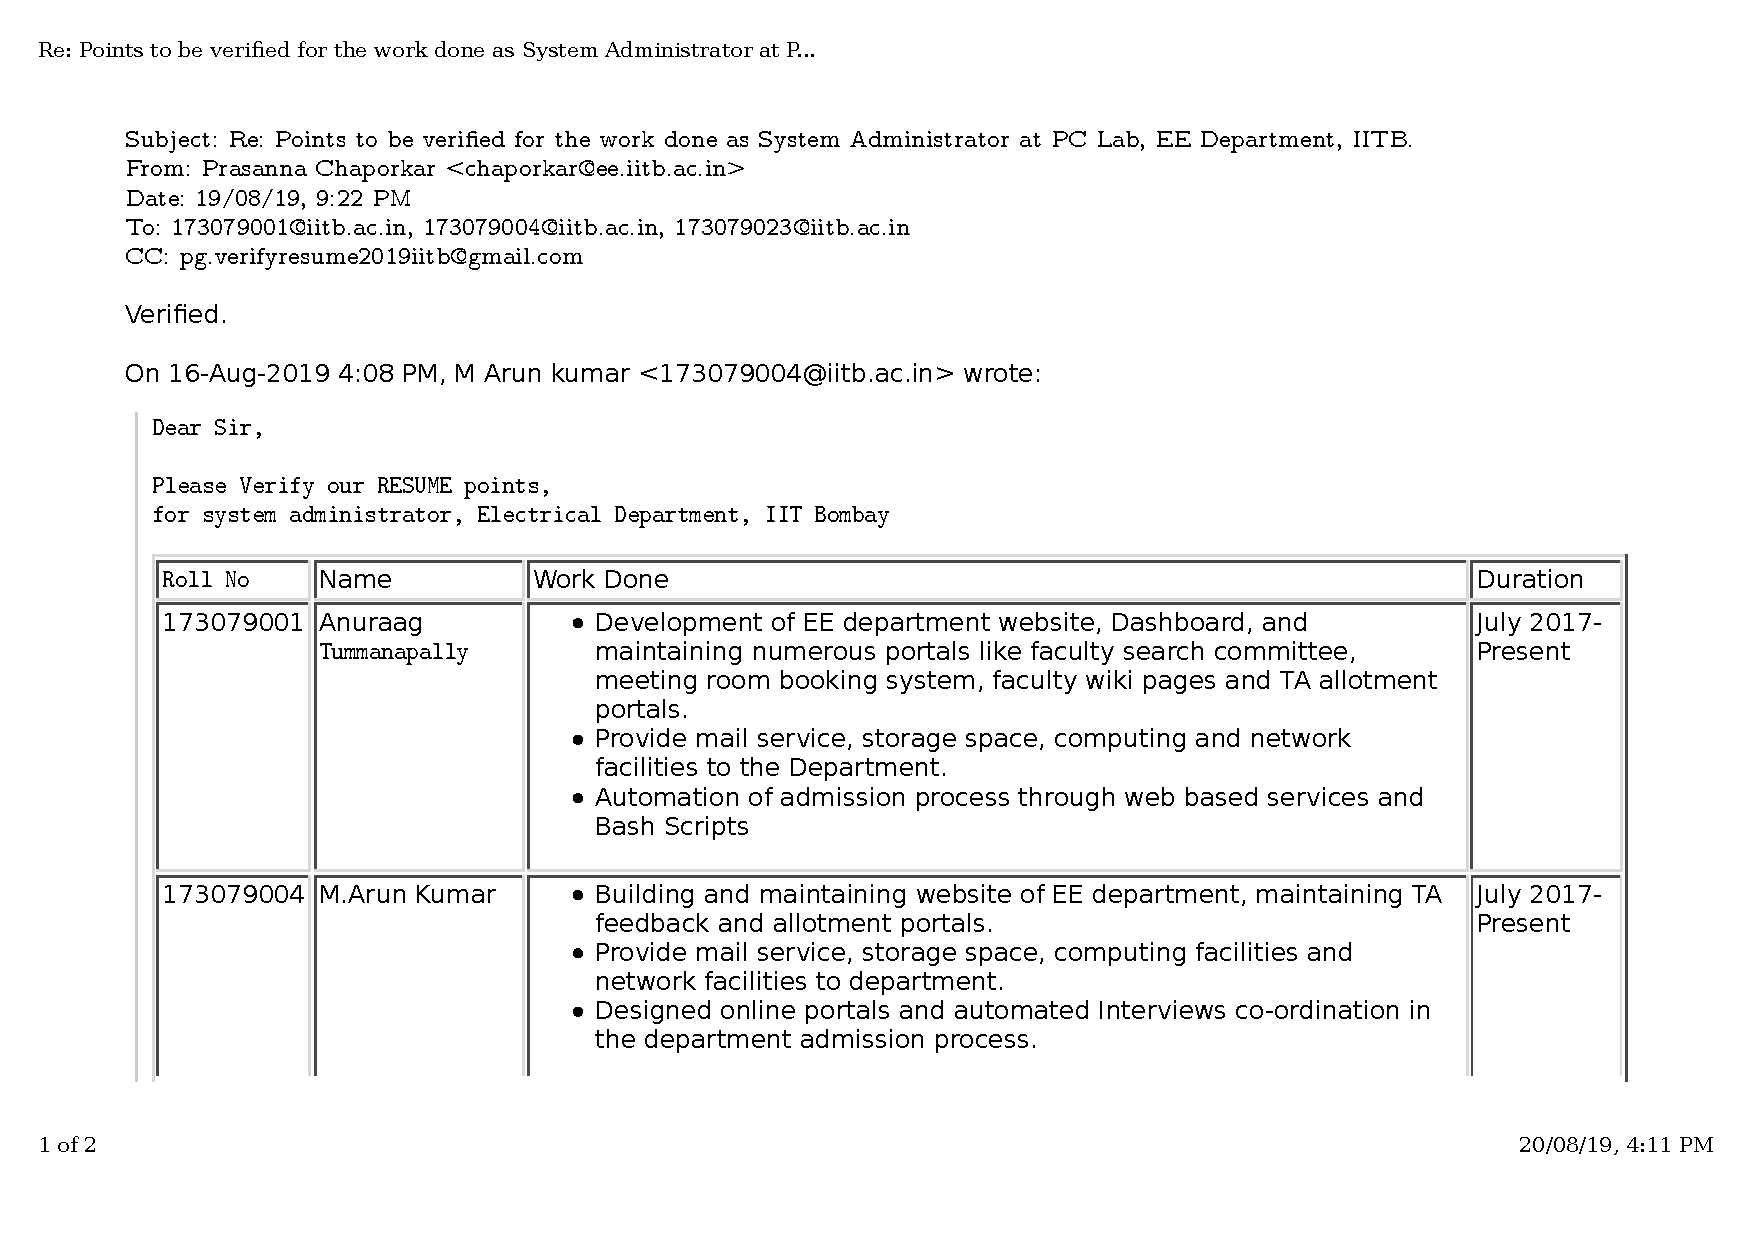
\includegraphics[trim={0 0 0 0},clip, width=\textwidth]{docs/sysad_work.pdf}}
		\end{figure}
\newpage
\section{Key Course Projects}
	\subsection{Verified By DPC}
	
\newpage
\section{Positions of Responsibility}
	\subsection{E-Mail from Hostel 1 Gen. Secy}
		For Web Secy in Hostel 1
		\begin{figure}[h]
			\frame{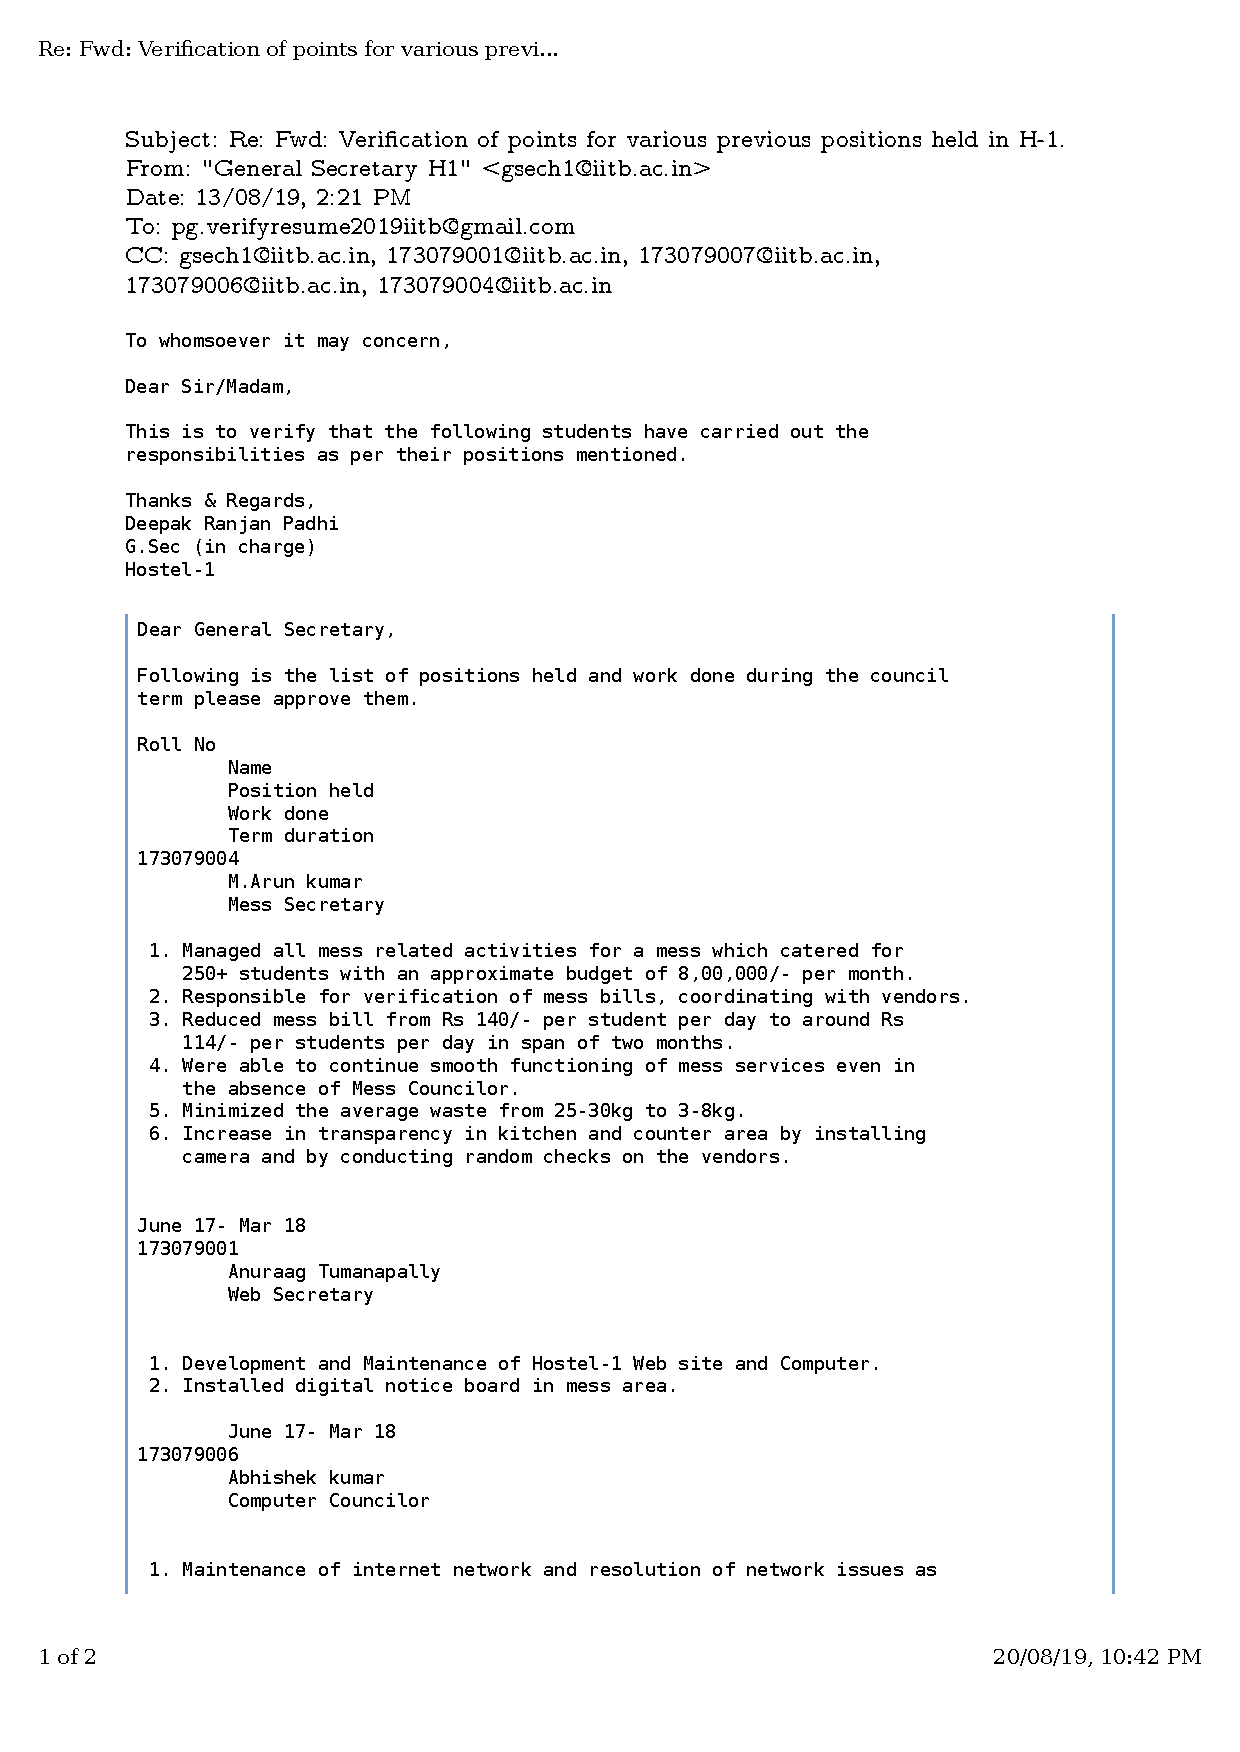
\includegraphics[trim={0 0 0 0},clip, width=0.8\textwidth]{docs/hostel1.pdf}}
		\end{figure}
\newpage
		\noindent For Web Secy in Hostel 1 continued..
		\begin{figure}[h]
			\frame{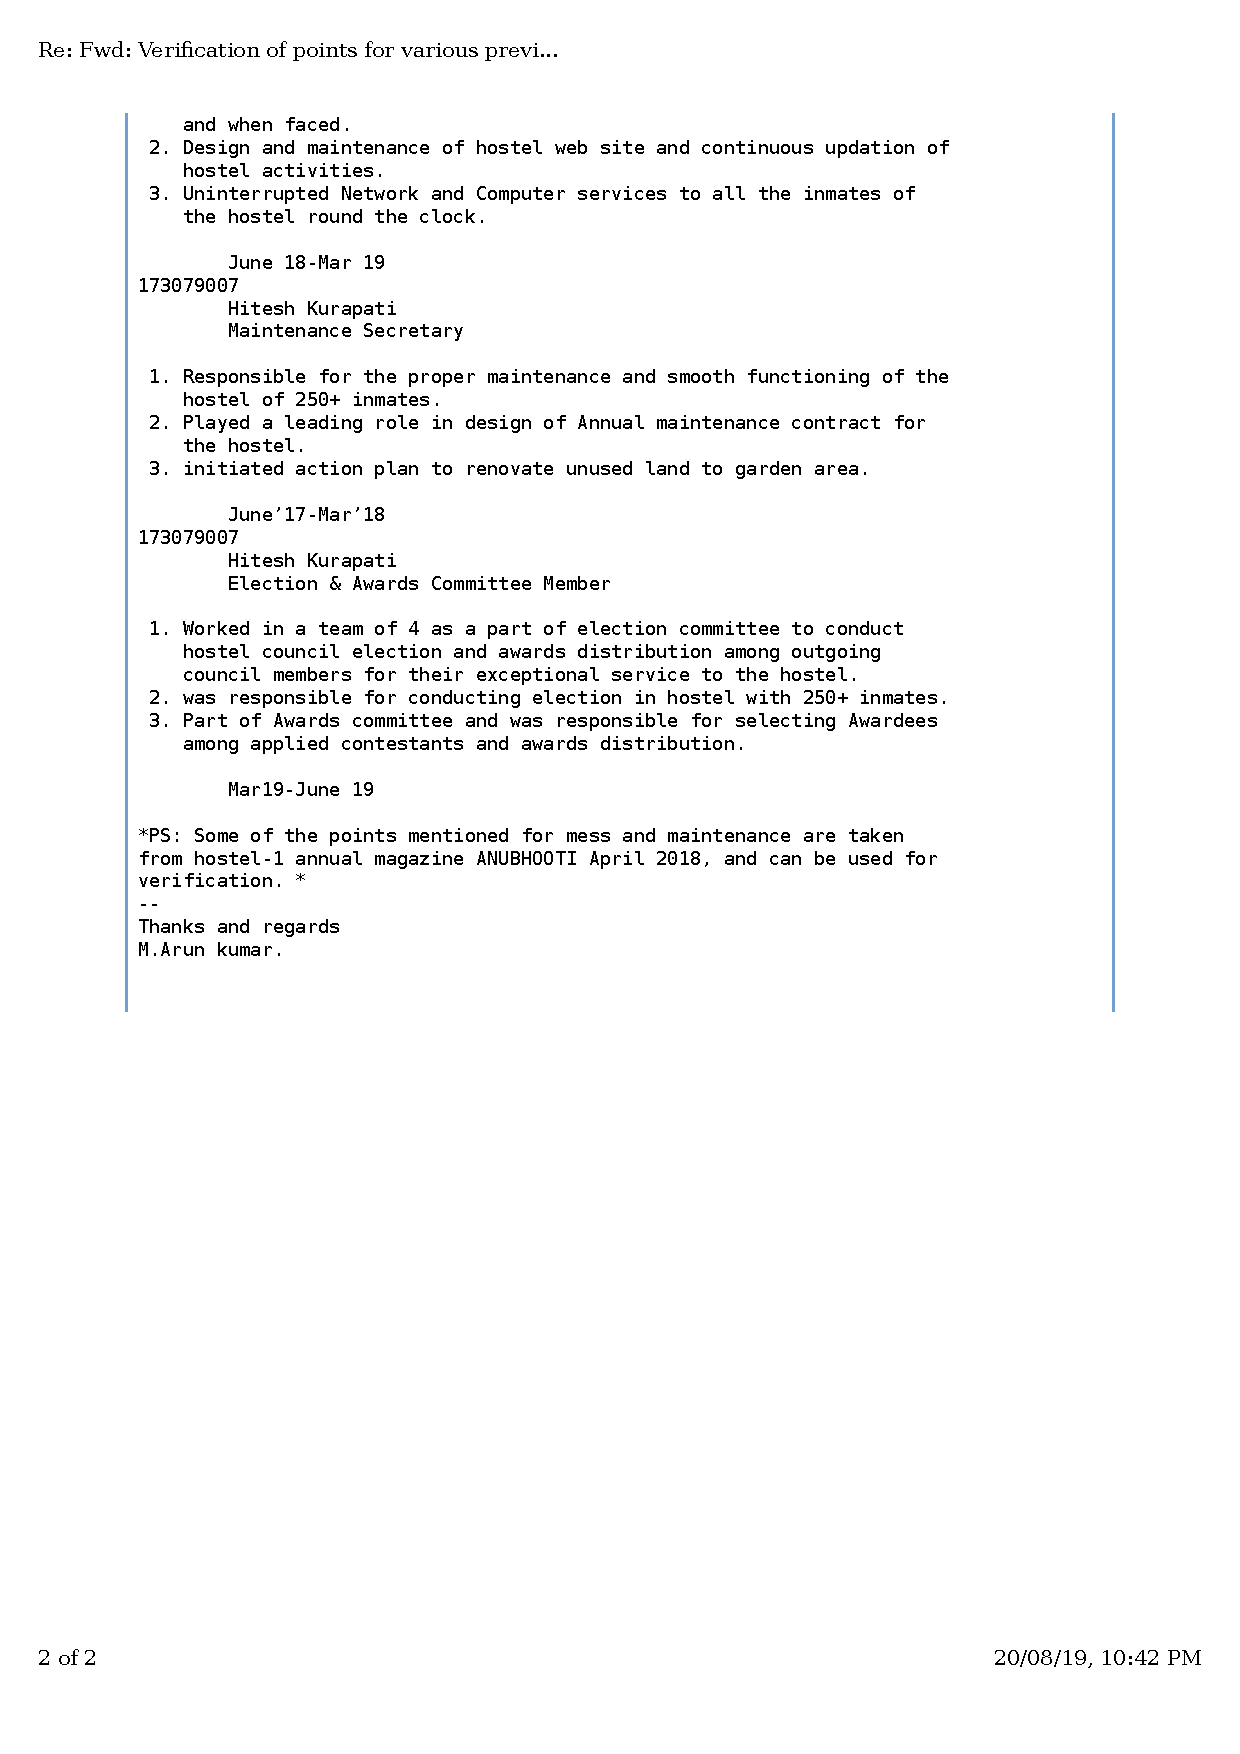
\includegraphics[trim={0 0 0 0},clip, width=0.8\textwidth]{docs/hostel1-pg2.pdf}}
		\end{figure}
\newpage
	\subsection{E-Mail from current OC, Bridgecourse}
		For Overall Coordinator, Bridgecourse
		\begin{figure}[h]
			\frame{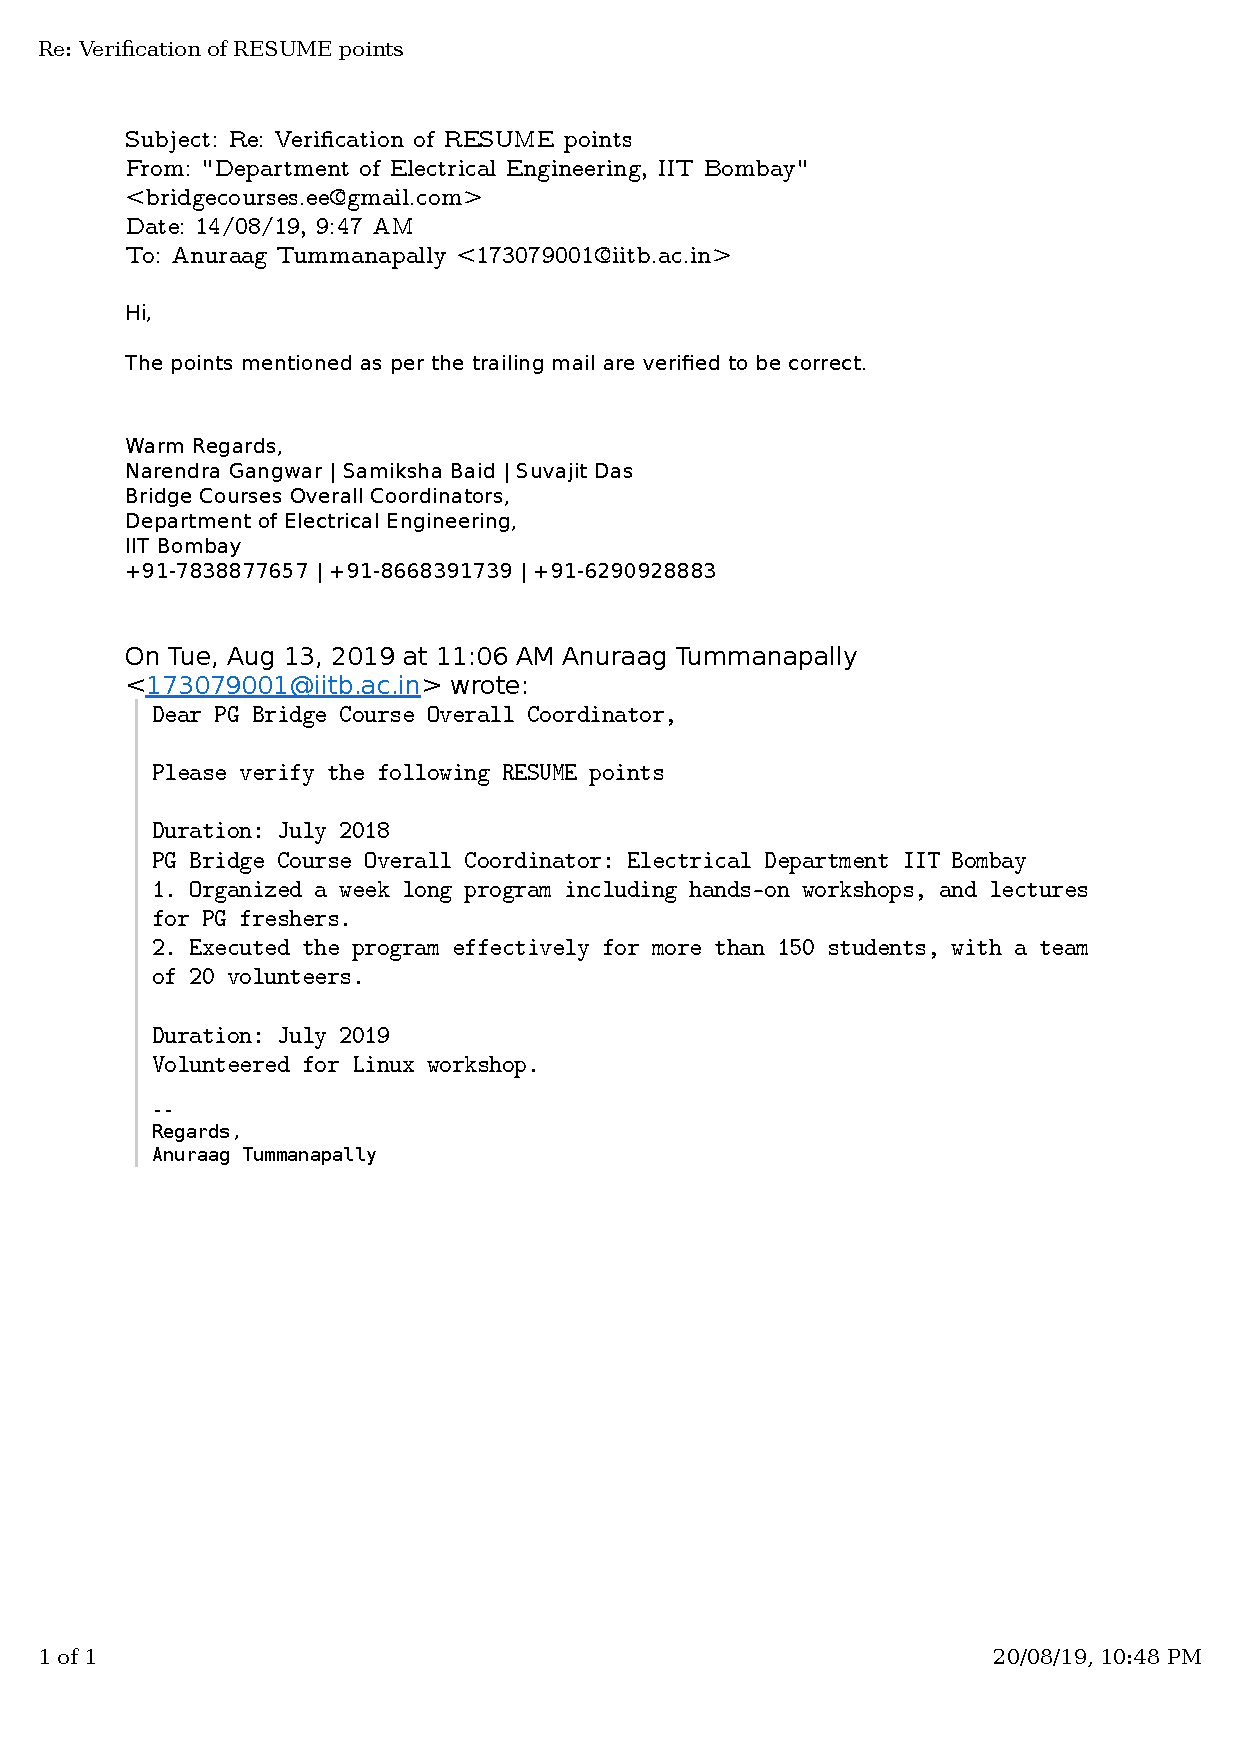
\includegraphics[trim={0 0 0 0},clip, width=0.8\textwidth]{docs/bridgecourses.pdf}}
		\end{figure}
\newpage
	\subsection{E-Mail from Faculty Coordinator, ISCP}

\newpage
	\subsection{E-Mail from PGAC Gen. Secy}
		For Web Nominee, PGAC
		\begin{figure}[h]
			\frame{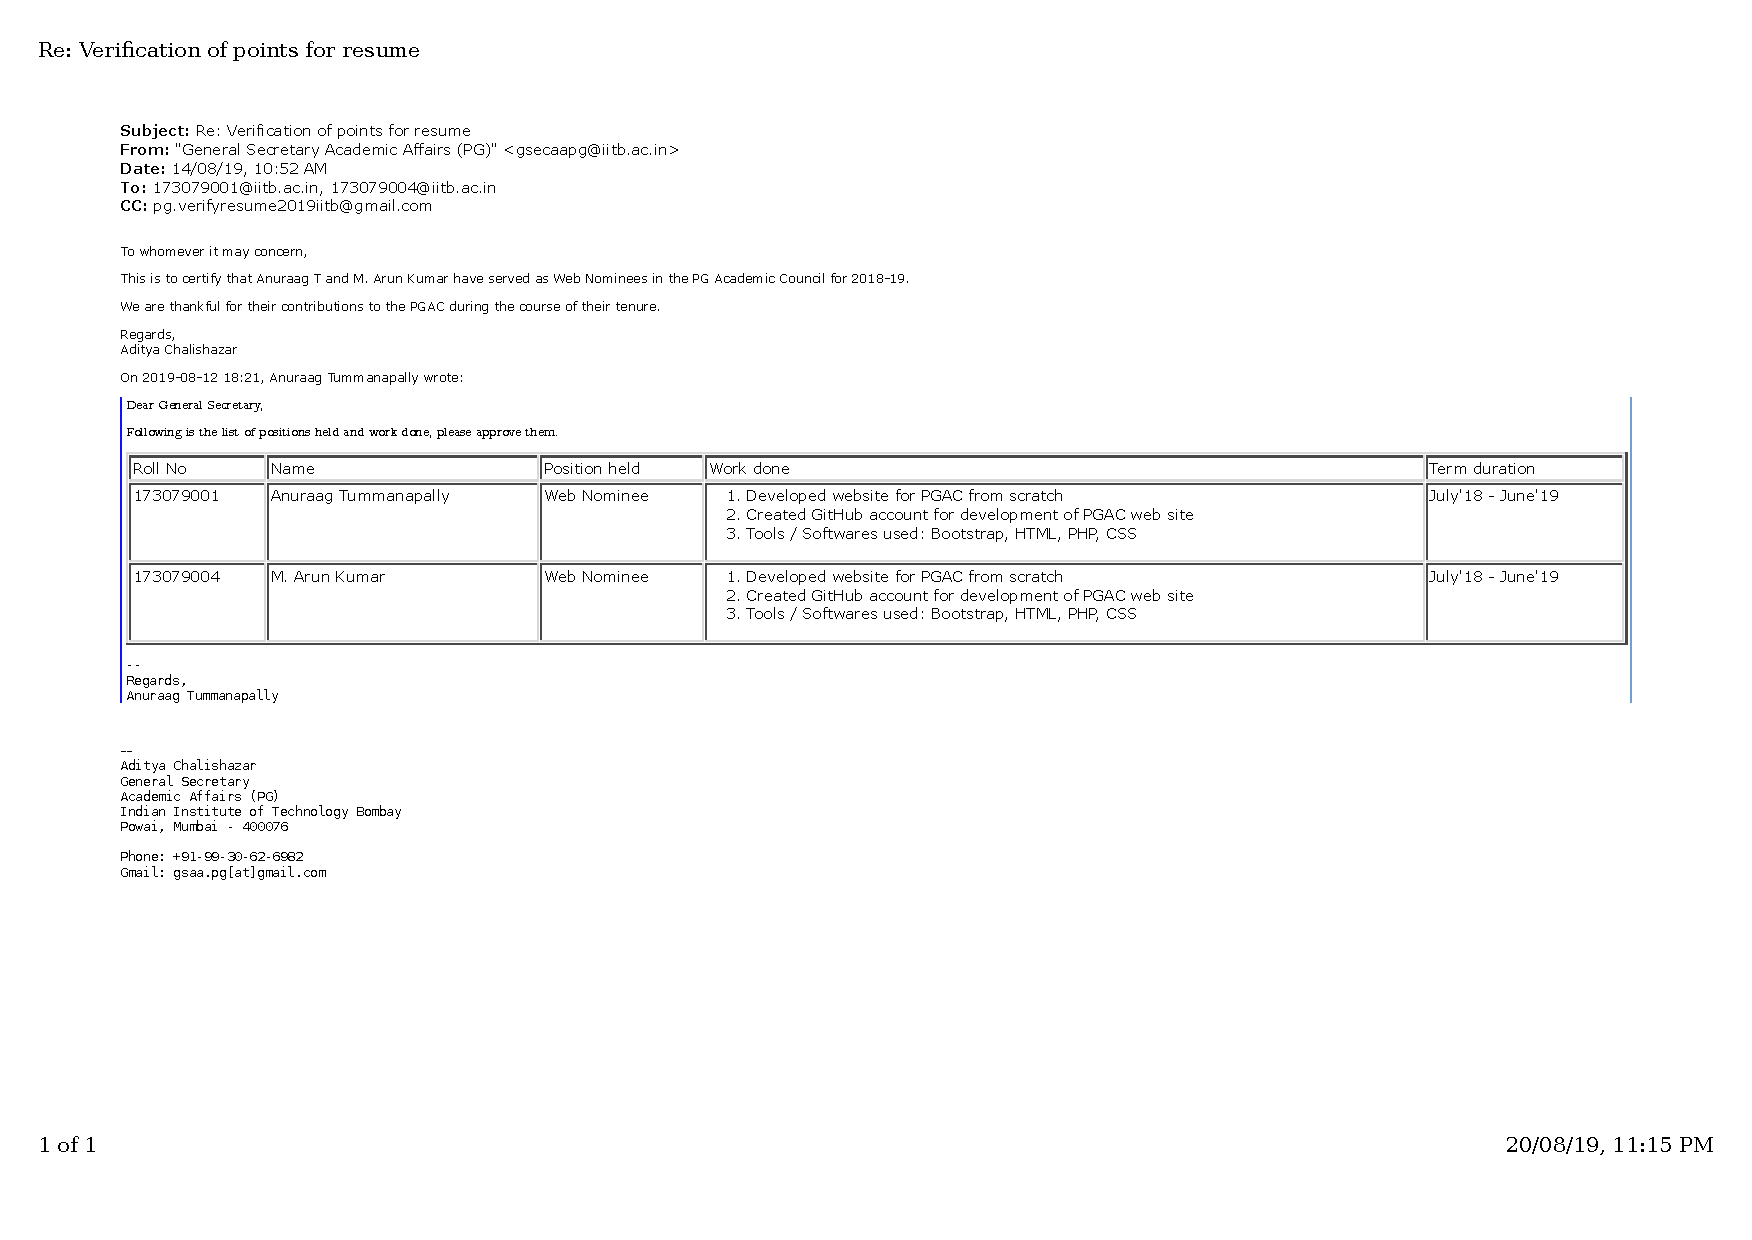
\includegraphics[trim={0 0 0 0},clip, width=\textwidth]{docs/pgac.pdf}}
		\end{figure}
\newpage
	\subsection{E-Mail from OC, SRG EE IITB}
		For Web Co-ordinator, SRG EE IITB 
		\begin{figure}[h]
			\frame{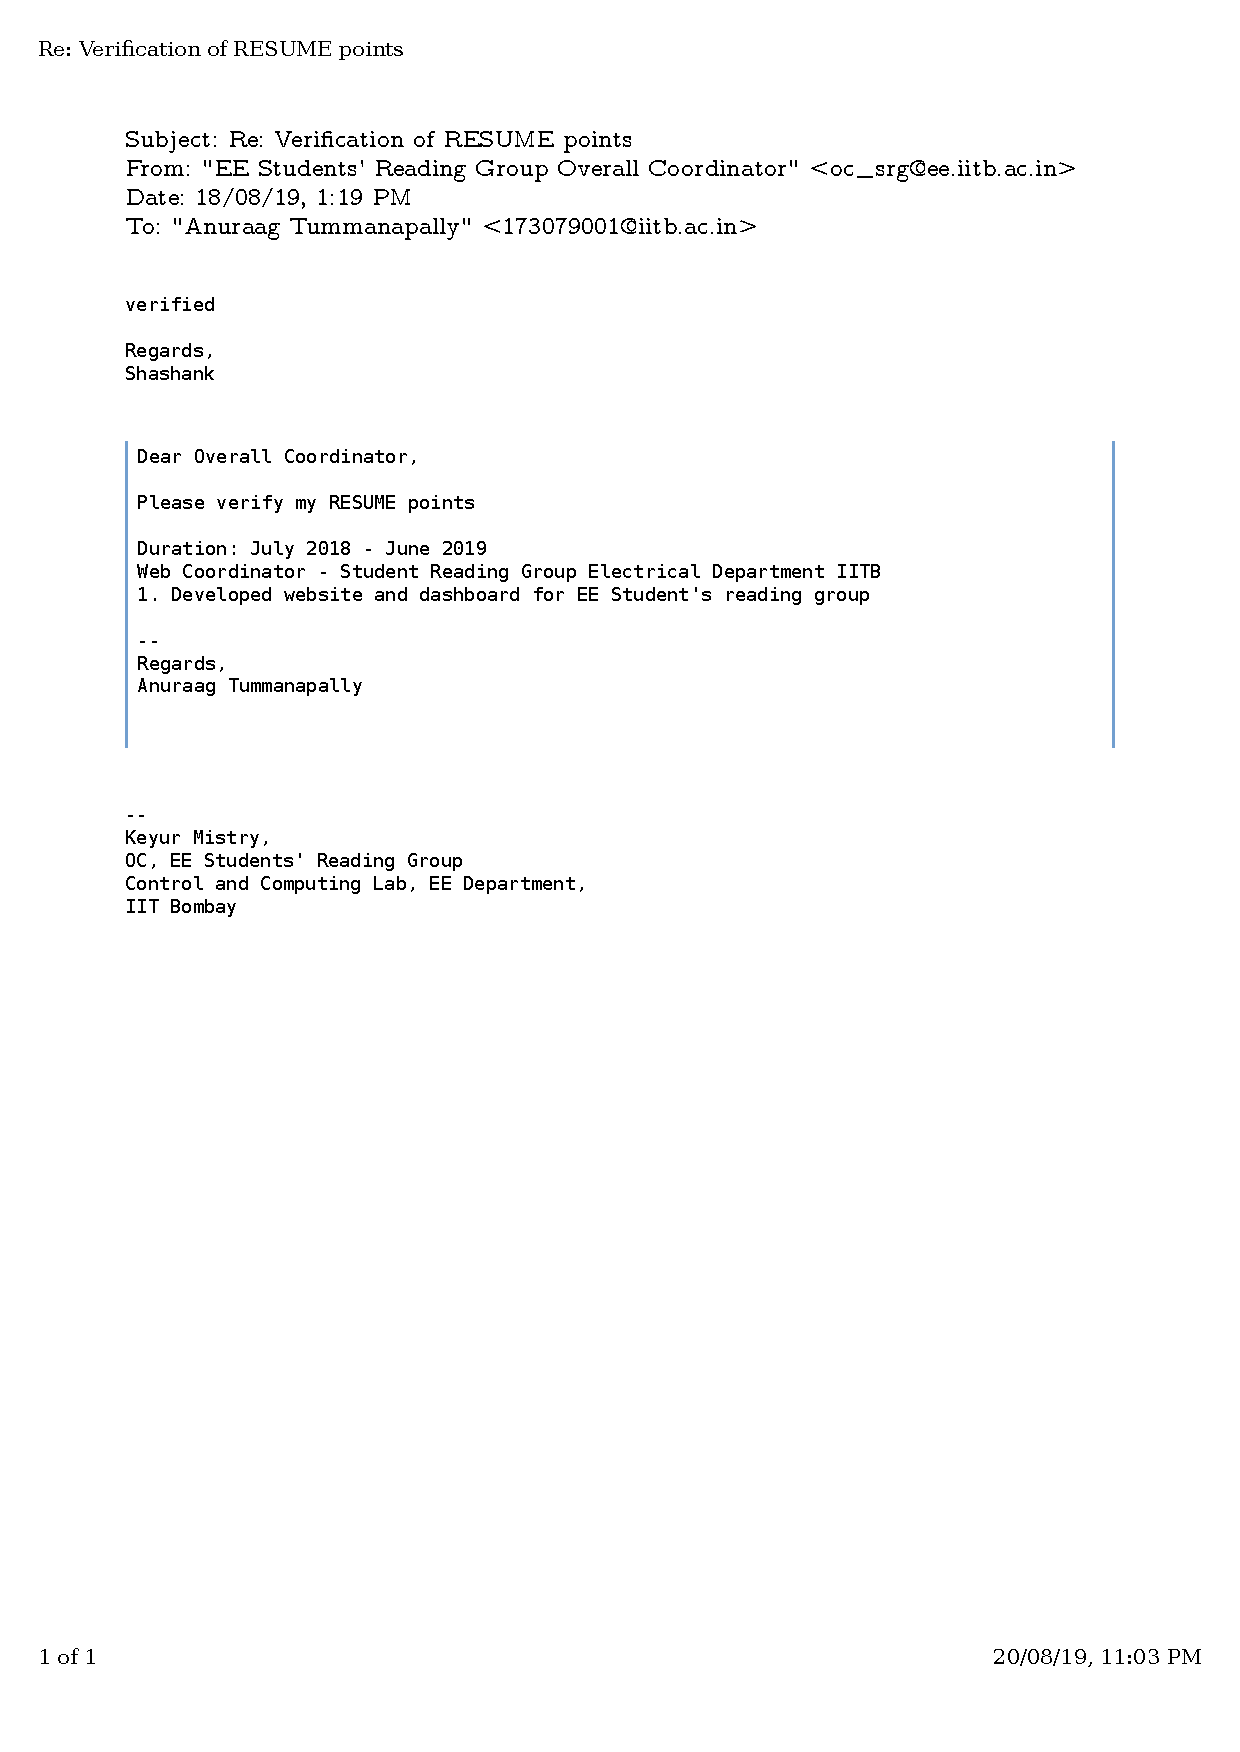
\includegraphics[trim={0 0 0 0},clip, width=0.8\textwidth]{docs/students_reading_group.pdf}}
		\end{figure}
\newpage
\section{Other Activities \& Interests}
	\subsection{Certificate from PGAC, IITB}
		For Volunteer, in Python workshop by PGAC
		\begin{figure}[h]
			\frame{
\includegraphics[trim={0 0 0 0},clip, width=0.8\textwidth]{docs/python_pgac.pdf}}
		\end{figure}

\newpage
	\subsection{E-Mail from current OC, Bridgecourse}
		For Linux session volunteering.
		\begin{figure}[h]
			\frame{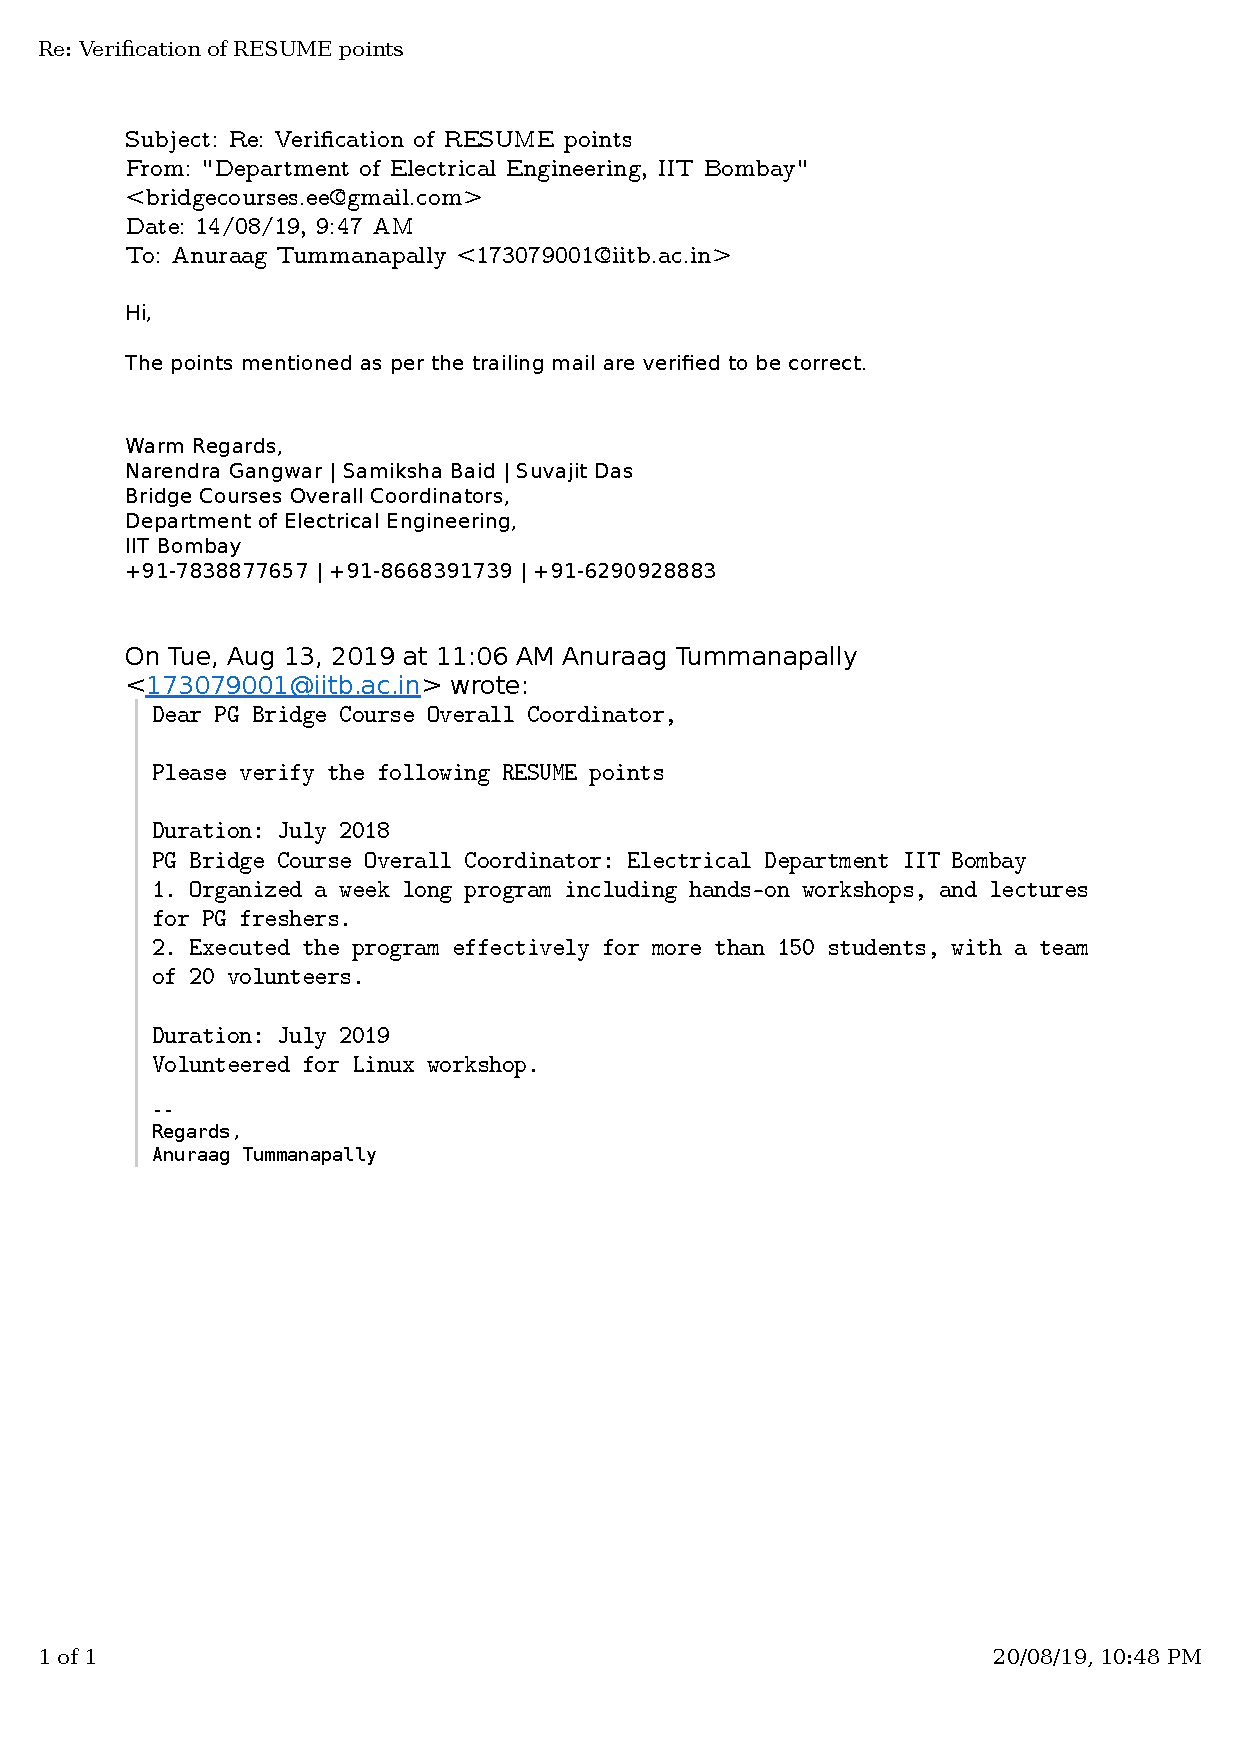
\includegraphics[trim={0 0 0 0},clip, width=0.8\textwidth]{docs/bridgecourses.pdf}}
		\end{figure}
\end{document}
